% Nicholas M. Rathmann <rathmann@nbi.ku.dk>

\documentclass[border=0pt,tikz]{standalone}

\usepackage{pgfplots,physics}
\usepackage{newtxtext,newtxmath} % RSPA-like font

\tikzset{
	lbl/.style={font=\fontsize{9.5}{9.5}\selectfont, inner sep=0},
	fig/.style={anchor=south west, inner sep=0}
}

\begin{document}
\begin{tikzpicture}[]

\node[fig] (A) at (0,0) {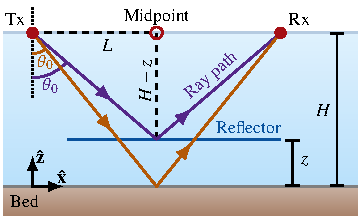
\includegraphics[scale=1]{../../schematics/CMP/solid.pdf}};

\node[fig] (B) at (6.3cm,-0.35cm) {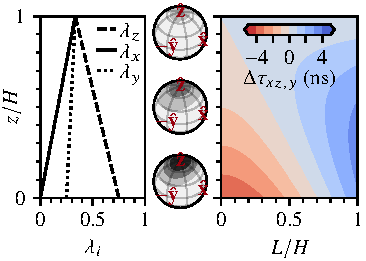
\includegraphics[scale=0.84]{CMP-solid.pdf}};

\gdef\xref{5.7cm}
\gdef\yref{3.45cm}
\node[lbl,anchor=west] at (\xref,\yref) {(a)};
\node[lbl,anchor=east] at (\xref+1.4cm,\yref) {(b)};
\node[lbl,anchor=west] at (\xref+3.6cm,\yref) {(c)};

\end{tikzpicture}

\end{document}